\documentclass{assignment}

\course{ECO 120-04}
\name{Lucas Reddinger}
\date{Wednesday 5 October 2022}
\doctitle{Assignment 4 Solutions}

\begin{document}
\RaggedRight

\beginsolutions{}

\section*{The U.S.~labor market}

\begin{enumerate}

\item Consider the U.S.~labor market, which is in equilibrium with wage $w_\text{2020q1}$ and quantity of labor $L_\text{2020q1}$. Depict this with a supply and demand model (as always, label axes and curves properly).

\begin{solution}
\begin{center}
\begin{tikzpicture}[scale=0.7]
\draw[thick,<->] (0,10) node[below left]{wage $w$}--(0,0)--(10,0) node[below right]{$L$ (hours)};
\draw[thick,red] (1,1)--(9,9) node[right]{$S$};
\draw[thick,blue] (1,9)--(9,1) node[right]{$D$};
\draw[dashed] (0,5) node[left]{$w_\text{2020q1}$} --(5,5) --(5,0) node[below]{$L_\text{2020q1}$};
\end{tikzpicture}
\end{center}
\end{solution}

\item Which entities (e.g., in the circular flow diagram) does the demand curve represent?

\begin{solution}
\emph{Complete answer:} Firms.

Firms demand labor and pay wages (which is the price of hourly labor).
\end{solution}

\item Which entities does the supply curve represent?

\begin{solution}
\emph{Complete answer:} Households.

Households supply labor and are paid wages for labor supplied.
\end{solution}

\item Suppose that due to the pandemic, people generally want to work less. On the same graph above, please illustrate this change and label any new curves with a subscript $1$.

\begin{solution}
Supply of labor in the U.S.~has decreased. In supply and demand diagrams, a decrease is represented by an inward shift (to the left).

\begin{center}
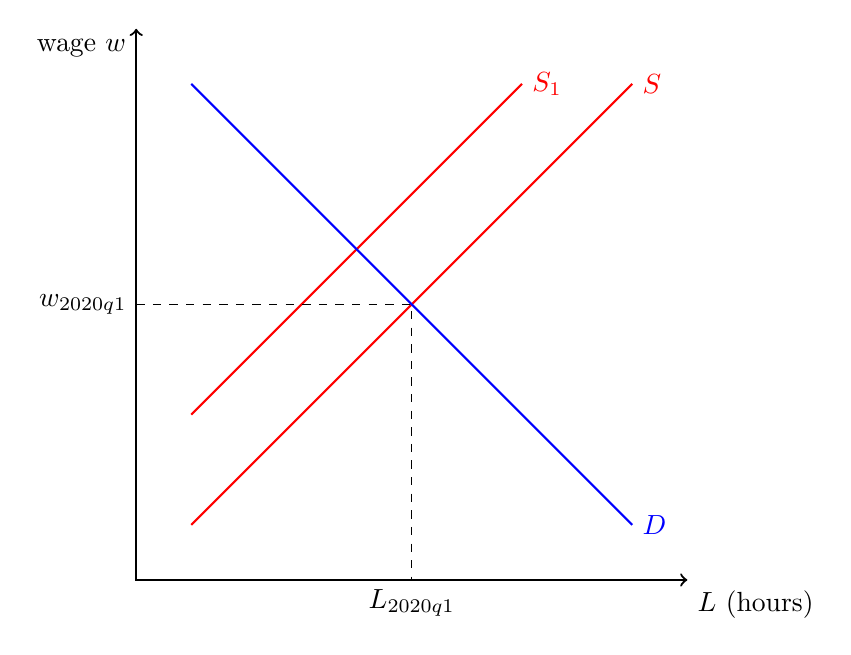
\begin{tikzpicture}[scale=0.7]
\draw[thick,<->] (0,10) node[below left]{wage $w$}--(0,0)--(10,0) node[below right]{$L$ (hours)};
\draw[thick,red] (1,1)--(9,9) node[right]{$S$};
\draw[thick,red] (1,3)--(7,9) node[right]{$S_1$};
\draw[thick,blue] (1,9)--(9,1) node[right]{$D$};
\draw[dashed] (0,5) node[left]{$w_\text{2020q1}$} --(5,5) --(5,0) node[below]{$L_\text{2020q1}$};
\end{tikzpicture}
\end{center}
\end{solution}

\item Because the pandemic has made international trade more difficult, U.S.~firms want to increase domestic production of goods. Accordingly, U.S.~firms want to hire additional labor. On the same graph above, please illustrate this change and label any new curves with a subscript $2$.

\begin{solution}
Demand of labor in the U.S.~has increased. In supply and demand diagrams, an increase is represented by an outward shift (to the right).

\begin{center}
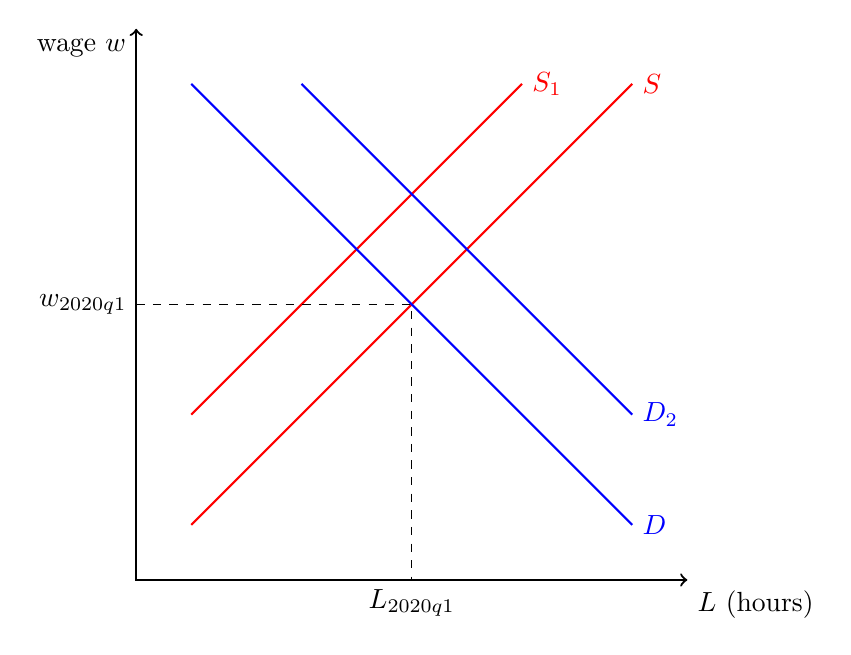
\begin{tikzpicture}[scale=0.7]
\draw[thick,<->] (0,10) node[below left]{wage $w$}--(0,0)--(10,0) node[below right]{$L$ (hours)};
\draw[thick,red] (1,1)--(9,9) node[right]{$S$};
\draw[thick,red] (1,3)--(7,9) node[right]{$S_1$};
\draw[thick,blue] (1,9)--(9,1) node[right]{$D$};
\draw[thick,blue] (3,9)--(9,3) node[right]{$D_2$};
\draw[dashed] (0,5) node[left]{$w_\text{2020q1}$} --(5,5) --(5,0) node[below]{$L_\text{2020q1}$};
\end{tikzpicture}
\end{center}
\end{solution}

\item Given all these changes to supply and demand, please label the new equilibrium wage as $w_\text{2021q1}$ and equilibrium quantity of labor traded as $L_\text{2021q1}$.

\begin{solution}
\begin{center}
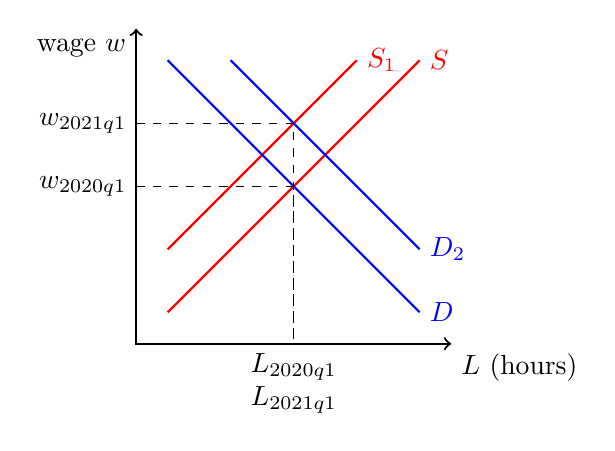
\begin{tikzpicture}[scale=0.4]
\draw[thick,<->] (0,10) node[below left]{wage $w$}--(0,0)--(10,0) node[below right]{$L$ (hours)};
\draw[thick,red] (1,1)--(9,9) node[right]{$S$};
\draw[thick,red] (1,3)--(7,9) node[right]{$S_1$};
\draw[thick,blue] (1,9)--(9,1) node[right]{$D$};
\draw[thick,blue] (3,9)--(9,3) node[right]{$D_2$};
\draw[dashed] (0,5) node[left]{$w_\text{2020q1}$} --(5,5) --(5,0) node[below]{$L_\text{2020q1}$};
\draw[dashed](0,7) node[left]{$w_\text{2021q1}$} --(5,7) --(5,0) node[below,yshift=-12pt]{$L_\text{2021q1}$};
\end{tikzpicture}
\end{center}
\vspace{-12pt}
\end{solution}

\item Do you know whether $L_\text{2021q1}$ is higher than, lower than, or the same as $L_\text{2020q1}$?

\begin{solution}
\emph{Complete answer:} The overall effect of these two changes on equilibrium labor is ambiguous.

One curve shift (supply shifting in) decreased labor traded. Another curve shift (demand shifting out) increased labor traded. Because these two shifts oppose each other in direction, we cannot determine the overall effect. We can easily shift each curve by different amounts to make the overall change in $L$ positive (below left), negative (below right), or equal (as already depicted above).

\begin{center}
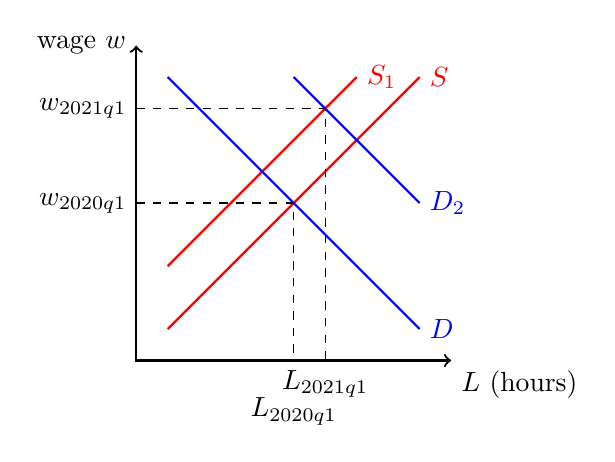
\begin{tikzpicture}[scale=0.4]
\draw[thick,<->] (0,10) node[left]{wage $w$}--(0,0)--(10,0) node[below right]{$L$ (hours)};
\draw[thick,red] (1,1)--(9,9) node[right]{$S$};
\draw[thick,red] (1,3)--(7,9) node[right]{$S_1$};
\draw[thick,blue] (1,9)--(9,1) node[right]{$D$};
\draw[thick,blue] (5,9)--(9,5) node[right]{$D_2$};
\draw[dashed] (0,5) node[left]{$w_\text{2020q1}$} --(5,5) --(5,0) node[below,yshift=-10pt]{$L_\text{2020q1}$};
\draw[dashed](0,8) node[left]{$w_\text{2021q1}$} --(6,8) --(6,0) node[below]{$L_\text{2021q1}$};
\end{tikzpicture}
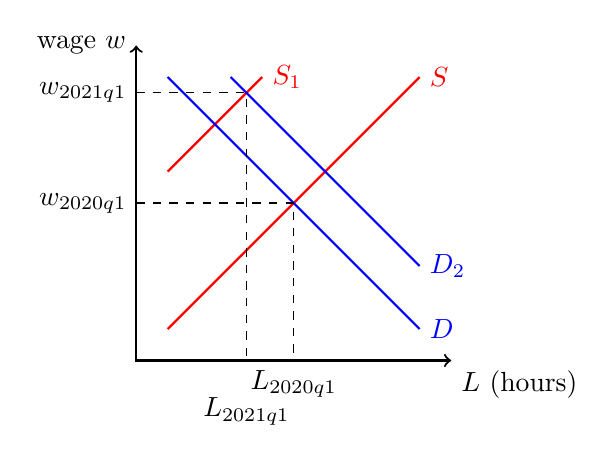
\begin{tikzpicture}[scale=0.4]
\draw[thick,<->] (0,10) node[left]{wage $w$}--(0,0)--(10,0) node[below right]{$L$ (hours)};
\draw[thick,red] (1,1)--(9,9) node[right]{$S$};
\draw[thick,red] (1,6)--(4,9) node[right]{$S_1$};
\draw[thick,blue] (1,9)--(9,1) node[right]{$D$};
\draw[thick,blue] (3,9)--(9,3) node[right]{$D_2$};
\draw[dashed] (0,5) node[left]{$w_\text{2020q1}$} --(5,5) --(5,0) node[below]{$L_\text{2020q1}$};
\draw[dashed](0,8.5) node[left]{$w_\text{2021q1}$} --(3.5,8.5) --(3.5,0) node[below,yshift=-10pt]{$L_\text{2021q1}$};
\end{tikzpicture}
\vspace{-12pt}
\end{center}

Clearly the change in $L$ is ambiguous, as it depends on the comparative magnitudes of the shifts of the two curves.
\end{solution}

\item Do you know whether $w_\text{2021q1}$ is higher than, lower than, or the same as $w_\text{2020q1}$?

\begin{solution}
\emph{Complete answer:} $w_\text{2021q1} > w_\text{2020q1}$.

One curve shift (supply shifting in) increased the equilibrium wage. Another curve shift (demand shifting out) also increased the equilibrium wage. Because these two shifts are in the same direction, we know that the wage must increase overall.
\end{solution}

\end{enumerate}

\end{document}
